\chapter{Plasma-Surface Interaction, Sputtering and Erosion}
\label{ch:pmi}

The preceding chapters established that a bounded plasma communicates with any material surface through a thin, non-neutral sheath, and that the surface receives a directed ion energy flux $\GammaE = \Gamma_i \langle E_i\rangle$ set by the Bohm current $\Gamma_i = n_s \uB$ and the mean impact energy $\langle E_i\rangle$ accumulated across the sheath potential fall. This chapter follows that flux across the plasma-solid boundary: ions transfer momentum to lattice atoms through collision cascades, ejecting sputtered neutrals; reactive species open chemical erosion channels a purely kinetic treatment cannot capture; energy not carried away by sputtered particles is deposited as heat, driving temperature rise, secondary electron emission, and eventually melting or cracking; and integrated erosion becomes the single most consequential quantity for electric-propulsion hardware, plasma-etched microstructures, and fusion plasma-facing components (PFCs) alike. Each consequence is a functional of $\GammaE$: yield, thermal load, and erosion rate are moments of the ion energy distribution function $f_i(v)$ delivered to the wall, weighted by the flux. Quantifying $\GammaE$ with fidelity is the load input to every model below.

\section{Physical Sputtering}
\label{sec:pmi-physical-sputtering}

\subsection{Collision Cascades and the Threshold Energy}

Physical sputtering is the ejection of target atoms by momentum transfer from an incident ion, with no chemical bond breaking beyond mechanical rupture of the surface binding potential. Over the energy range of interest to sheath-accelerated ions (roughly \SIrange{1}{1000}{\electronvolt}), nuclear (elastic) collisions dominate: the ion initiates a collision cascade in which struck lattice atoms recoil, collide with neighbours, and redistribute the incoming energy through the near-surface region on a picosecond timescale \cite{ref0143,ref0144}. Sputtering occurs whenever cascade energy reaches a surface atom with outward momentum sufficient to overcome $U_0$.

A minimal kinematic picture already fixes the existence of a threshold. Treating the primary encounter as a binary elastic collision between hard spheres, the maximum energy transferable to a target atom at rest is
\begin{equation}
T_{\max} = \gamma E, \qquad \gamma \equiv \frac{4 M_1 M_2}{(M_1+M_2)^2},
\label{eq:pmi-gamma}
\end{equation}
where $\gamma \le 1$ is maximised at $\gamma=1$ for mass-matched partners and falls off for asymmetric masses. For an atom to be ejected it must receive, after cascade losses, at least $U_0$ directed outward; the incident energy at which this first becomes kinematically possible defines the threshold energy,
\begin{equation}
E_{\mathrm{th}} \sim \frac{U_0}{\gamma} = \frac{U_0 (M_1+M_2)^2}{4 M_1 M_2}.
\label{eq:pmi-ethreshold}
\end{equation}
Equation~\eqref{eq:pmi-ethreshold} is a lower bound: real cascades lose energy to multiple sub-threshold collisions before any atom escapes, so the true threshold sits a factor of a few above this minimum. For light ions on heavy targets ($M_1 \ll M_2$), $\gamma \to 4M_1/M_2$ is small and the threshold correspondingly high, which is why hydrogenic ions on tungsten -- the reference PFC material for fusion -- show thresholds on the order of hundreds of electronvolts (roughly 150-450 eV depending on isotope) despite tungsten's low yield at typical divertor energies \cite{ref0158,ref0189}. Below $E_{\mathrm{th}}$, only chemical or thermally activated channels (Section~\ref{sec:pmi-chemical}) can erode the surface. Measured thresholds for low-energy argon and neon ions on metals confirm the mass-ratio scaling qualitatively, with fitted values typically \SIrange{2}{8}{\electronvolt} above the kinematic value depending on crystallographic orientation \cite{ref0152}.

\subsection{The Sigmund Linear-Cascade Theory}

The quantitative theory of sputtering yield in the collision-cascade regime is due to Sigmund, who treated the cascade as a linear transport problem: each collision involves only two bodies, electronic-excitation losses are treated separately from nuclear stopping, and the density of recoiling atoms arriving at the surface follows from Boltzmann transport theory \cite{ref0143,ref0144}. The central result: yield -- mean atoms ejected per incident ion -- is proportional to the nuclear stopping power $S_n(E)$ and inversely proportional to the surface binding energy:
\begin{equation}
Y(E) = \Lambda \,\alpha\!\left(\frac{M_2}{M_1}\right) \frac{S_n(E)}{U_0},
\label{eq:pmi-sigmund}
\end{equation}
where $\Lambda$ collects normal-incidence numerical and density constants, and $\alpha(M_2/M_1)$ is a slowly varying function of mass ratio -- order $0.1$--$0.2$ for $M_2/M_1 \lesssim 1$, rising toward unity as $M_2/M_1$ increases -- encoding how efficiently momentum backscatters toward the surface \cite{ref0143}. The nuclear stopping power follows from a screened-Coulomb potential; in the universal Lindhard--Thomas--Fermi reduction it is written in terms of a reduced energy $\epsilon$,
\begin{equation}
\epsilon = \frac{a\,M_2}{Z_1 Z_2 e^2 (M_1+M_2)}\,E, \qquad
S_n(E) = \frac{4\pi Z_1 Z_2 e^2 a}{M_1/M_2+1}\; s_n(\epsilon),
\label{eq:pmi-stoppingpower}
\end{equation}
with $a$ the Firsov/Lindhard screening length, $Z_1,Z_2$ the atomic numbers, and $s_n(\epsilon)$ a universal reduced stopping function rising from zero, peaking near $\epsilon\sim0.3$--$1$, and falling off at high $\epsilon$ as electronic stopping takes over. Equation~\eqref{eq:pmi-sigmund} remains the workhorse model and anchors essentially all sputtering-yield tabulations used in propulsion, etching, and fusion engineering.

\subsection{Energy Dependence of the Yield}

Sigmund's result is asymptotically valid at moderate to high energy where $S_n(E)$ is well described by the universal function; it does not reproduce the vanishing of the yield at $E_{\mathrm{th}}$, since $S_n(E)$ stays finite at arbitrarily low energy. A widely used semi-empirical extension, due to Bohdansky, multiplies the Sigmund yield by a threshold factor fitted to low-energy data:
\begin{equation}
Y(E) = Q\, S_n(E) \left[1-\left(\frac{E_{\mathrm{th}}}{E}\right)^{2/3}\right]\left[1-\frac{E_{\mathrm{th}}}{E}\right]^{2}, \qquad E > E_{\mathrm{th}},
\label{eq:pmi-bohdansky}
\end{equation}
and $Y(E)=0$ for $E \le E_{\mathrm{th}}$, where $Q$ is a fitted constant absorbing $\Lambda\alpha/U_0$. Equation~\eqref{eq:pmi-bohdansky} reproduces three features seen across ion-target combinations: a hard threshold at $E_{\mathrm{th}}$; a steep, super-linear rise above it; and a broad maximum at intermediate energy (hundreds of eV to a few keV for light noble-gas ions on metals) followed by a slow decline as a smaller cascade fraction reaches the surface \cite{ref0144}. Systematic yield measurements for low-energy \ce{Ar+} and \ce{Ne+} ions on metals confirm this shape and supply the fitted constants $(Q, E_{\mathrm{th}})$ used throughout the erosion-modelling literature \cite{ref0152}. On multi-element surfaces the yield is not a linear combination of elemental yields weighted by surface concentration: preferential sputtering of the lower-$U_0$ constituent depletes it near the surface, so steady-state and transient yields differ as composition evolves -- relevant wherever the PFC is not a pure element, e.g. stainless-steel walls or multi-element propellant-grid alloys.

Because the ion energy delivered to a wall is distributed, not monoenergetic, the relevant yield is the flux-weighted average
\begin{equation}
\langle Y \rangle = \frac{1}{\Gamma_i}\int_0^\infty Y(E)\, \frac{d\Gamma_i}{dE}\, dE,
\label{eq:pmi-yieldaverage}
\end{equation}
where $d\Gamma_i/dE$ is the differential ion energy flux at the surface, obtained by projecting $f_i(v)$ through the sheath acceleration onto the energy axis. Because $Y(E)$ is strongly convex near $E_{\mathrm{th}}$, the high-energy tail of the distribution -- rather than its mean -- can dominate $\langle Y\rangle$ in low-temperature discharges where the bulk sits near or below threshold; this is a principal reason a kinetic characterisation of the ion flux, rather than the single fluid moment $\langle E_i\rangle$, is needed for accurate erosion prediction.

\subsection{Angular Dependence of the Yield}

Sheath-accelerated ions rarely strike a surface exactly along its normal: roughness, magnetic pre-sheath deflection, and tilted electrodes (grids, sidewalls, divertor targets) impose a distribution of incidence angles $\theta$. The angular dependence is described empirically by the Yamamura formula,
\begin{equation}
Y(\theta) = Y(0)\,(\cos\theta)^{-f}\, \exp\!\left[-\Sigma\!\left(\frac{1}{\cos\theta}-1\right)\right],
\label{eq:pmi-yamamura}
\end{equation}
where $f$ is an order-unity exponent controlling the initial rise with obliquity, and $\Sigma$ is a positive parameter (increasing with roughness and with $U_0/E$) suppressing the yield at grazing incidence. At oblique incidence the projected range shrinks as $\cos\theta$, so a larger cascade fraction ejects surface atoms and the yield rises above $Y(0)$. Beyond an optimum angle $\theta_{\mathrm{opt}}$, typically \SIrange{60}{80}{\degree} for keV-range ions on metals, a growing fraction of ions is reflected before penetrating far enough to initiate a cascade, and the yield falls sharply toward zero as $\theta \to \SI{90}{\degree}$. Where the magnetic field and sheath impose a narrow, field-aligned incidence angle -- magnetised divertor sheaths or Hall-thruster channel walls -- this angular law is the dominant lever by which geometry, not energy, sets local erosion; channel-wall erosion asymmetries in Hall thrusters follow directly \cite{ref0425,ref0433}.

\begin{figure}[htbp]
\centering
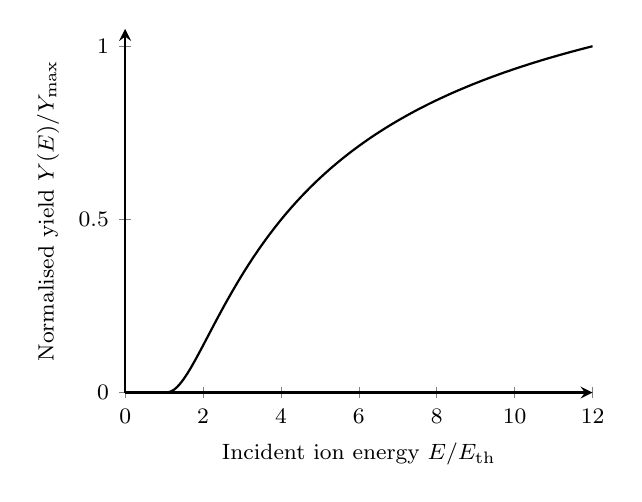
\begin{tikzpicture}
\begin{axis}[
 width=0.62\linewidth, height=6.2cm,
 xlabel={Incident ion energy $E/E_{\mathrm{th}}$},
 ylabel={Normalised yield $Y(E)/Y_{\max}$},
 xmin=0, xmax=12, ymin=0, ymax=1.05,
 domain=1:12, samples=200,
 axis lines=left,
 grid=none,
 tick label style={font=\footnotesize},
 label style={font=\footnotesize},
 line width=0.9pt,
]
\addplot[black, thick] {(1-(1/x)^(2/3))*(1-1/x)^2 / 0.68};
\end{axis}
\end{tikzpicture}
\caption{Schematic, illustrative curve of the Bohdansky-type threshold factor $[1-(E_{\mathrm{th}}/E)^{2/3}][1-E_{\mathrm{th}}/E]^{2}$ that multiplies the Sigmund nuclear-stopping yield, plotted against $E/E_{\mathrm{th}}$ and normalised to its own maximum over the plotted range. The curve is an analytic model, not measured or fitted data; it illustrates only the qualitative threshold-rise shape discussed in the text.}
\label{fig:pmi-yield-energy}
\end{figure}

Figure~\ref{fig:pmi-yield-energy} plots the dimensionless threshold factor of Equation~\eqref{eq:pmi-bohdansky} against $E/E_{\mathrm{th}}$, purely to illustrate the near-threshold rise; the true energy dependence of $Y(E)$ also carries the slowly varying $S_n(E)$ prefactor, not included in the plot.

\section{Chemical and Reactive Sputtering; Redeposition}
\label{sec:pmi-chemical}

\subsection{Chemically Enhanced Erosion}

Physical sputtering is switched off below $E_{\mathrm{th}}$, which can be tens of electronvolts for light-ion/heavy-target combinations. Many technologically important plasmas contain chemically reactive species -- oxygen, fluorine, hydrogen, and their radical derivatives -- that erode a surface by forming volatile compounds with the substrate, independent of or synergistically with ion bombardment. In chemical sputtering proper, a reactive species first forms a weakly bound surface complex; a subsequent, sub-threshold ion impact supplies enough activation energy to desorb it as a volatile molecule, so erosion proceeds well below the physical threshold with a yield that can exceed the purely physical value at the same energy. This is not confined to hydrocarbon chemistry: oxygen ion bombardment of metals produces enhanced yields, through oxide-layer formation and preferential removal of the more volatile oxidised species, and a substantial secondary-ion yield, since the electronegative oxygen adlayer lowers the ionisation barrier for sputtered atoms leaving as ions -- so measurements of only neutral or only ionised flux will systematically misestimate total erosion unless the ionised fraction is independently characterised.

A further complication: total yield per incident molecular ion is not additive in the constituent atomic yields, since correlated, closely spaced energy deposition into the same cascade produces a yield enhancement -- often superlinear in atom number -- relative to the sum expected from separate atomic ions. This is particularly relevant to hydrocarbon and hydrogen sputtering of carbon-based PFCs, and generally wherever the dominant species is molecular or a cluster ion. Physical and chemical channels are thus not simply additive; beam studies combining simultaneous ion and reactive-neutral exposure with single-channel reference measurements find synergistic enhancement factors of several times the naive sum, since ion bombardment continuously refreshes reactive sites that would otherwise passivate under neutral exposure alone.

\subsection{Redeposition and Net Erosion}

Sputtered and chemically eroded material does not vanish: it enters the plasma or vacuum environment as neutrals, molecules, and ions, a fraction of which is subsequently transported by plasma fields and neutral gas flow and redeposited elsewhere. The quantity of practical consequence is therefore never the gross yield $Y(E,\theta)$ alone but the \emph{net} erosion rate,
\begin{equation}
\Gamma_{\mathrm{net}}(\mathbf{r}) = \Gamma_{\mathrm{sputtered}}(\mathbf{r}) - \Gamma_{\mathrm{redeposited}}(\mathbf{r}).
\label{eq:pmi-neterosion}
\end{equation}
Redeposition is intrinsically a transport problem, coupling the local erosion source to the global plasma and neutral-gas flow field, and can differ dramatically between locations on the same component: regions with direct line of sight to the eroding surface accumulate redeposited material and can show net growth, while shadowed regions erode close to the gross rate. Studies of full-tungsten tokamak divertors illustrate this asymmetry starkly: gross erosion computed from ion energy flux and yield alone can overstate net material loss by a large factor where prompt redeposition is strong \cite{ref0158}. Because net, not gross, erosion limits lifetime, erosion-lifetime engineering (Section~\ref{sec:pmi-erosion-integral}) must generally couple to a redeposition model rather than be treated as purely local.

\section{Surface Heating, Thermal Loading and Secondary Electron Emission}
\label{sec:pmi-heating}

\subsection{Power Deposition by the Ion Energy Flux}

Sputtering removes only a small fraction, typically well under one percent by energy, of the power an ion delivers on impact; the great majority of $\GammaE$ is deposited as heat, through electronic and nuclear stopping, recombination with a surface electron, and the kinetic energy of secondary particles that do not escape. The surface heat flux is therefore, to good approximation, the ion energy flux itself, augmented by the electron heat flux and ionisation-potential release, reduced only marginally by sputtering and secondary-emission losses:
\begin{equation}
q_{\mathrm{surf}} \simeq \GammaE + \Gamma_i\, E_{\mathrm{iz}} + q_{e} - q_{\mathrm{SEE}} - q_{\mathrm{sput}},
\label{eq:pmi-heatbalance}
\end{equation}
where $E_{\mathrm{iz}}$ is the ionisation energy released on recombination, $q_e$ the electron contribution, and $q_{\mathrm{SEE}}$, $q_{\mathrm{sput}}$ the small losses to secondary electrons and sputtered particles. Because $\GammaE$ typically dominates Equation~\eqref{eq:pmi-heatbalance} in ion-bombarded, low-electron-temperature sheaths, direct measurement of surface heat flux gives an independent calorimetric check on the flux inferred from sheath-theoretic or probe diagnostics; heat-flux microsensors embedded in test surfaces have been used for this \cite{ref0175}. In magnetic-confinement geometries, where the flux is concentrated by field-line mapping onto narrow divertor strike regions, the resulting heat flux can dominate thermal response even for modest upstream parameters; distributing this load is a primary design driver \cite{ref0581}.

\subsection{Secondary Electron Emission and its Feedback on the Sheath}

Ion, and separately electron, bombardment releases secondary electrons through several mechanisms: potential (Auger neutralisation) emission, with no kinetic-energy threshold; kinetic emission, requiring a minimum impact energy; and, for electron-bombarded surfaces, true secondary emission from inelastic scattering. The yield $\gamma_{\mathrm{SE}}$ depends on ion species, charge state, impact energy and angle, surface composition, and -- critically for hot PFC surfaces -- temperature, since thermionic emission adds to the impact-driven yield. Secondary emission is not a passive loss channel: emitted electrons are accelerated back into the plasma by the same sheath potential that accelerated the ions inward, and a large $\gamma_{\mathrm{SE}}$ modifies the sheath's charge balance and potential profile. At surfaces hot enough to emit copiously, the outward electron current can approach or exceed the inward ion current, and the resulting "inverse" sheath changes the near-surface field and hence the effective ion impact energy for sputtering \cite{ref0038}. This feedback loop -- flux heats the surface, the hot surface modifies the sheath, and the modified sheath resets the flux -- means thermal loading and sputtering cannot, in the high-heat-flux limit, be treated as independent outputs of a fixed sheath, a concern for refractory metal PFCs.

\subsection{Transient and Steady-State Thermal Loads}

Two thermal-loading regimes must be distinguished. In steady-state operation the flux is approximately constant over timescales long compared with the thermal diffusion time, and surface temperature rises to a value set by the balance between incident heat flux and conductive (and, at high temperature, radiative) removal; actively cooled PFCs are designed around distributing this non-uniform flux to avoid hot spots \cite{ref0581}. In transient operation -- disruptions and ELMs, arcing, or pulsed thruster discharges -- the ion energy flux can rise by orders of magnitude over millisecond timescales, delivering an energy density far exceeding what steady-state conduction can remove; a small diffusion length means transient loads deposit in a thin layer, producing steep gradients and severe stress even when the time-averaged flux is modest. Pulsed electrothermal-discharge experiments reproducing disruption-like heat loads separate transient melt/vaporisation erosion from quasi-steady sputtering, since the two scale differently with pulse energy density \cite{ref0176}. Molecular-dynamics simulations further show the yield is not temperature-independent: a hotter lattice has reduced effective binding and altered defect mobility, so the same incident energy gives a different yield on a pre-heated surface, closing a second feedback loop linking thermal loading back to sputtering.

\section{Erosion as the Integral of the Ion Energy Flux}
\label{sec:pmi-erosion-integral}

\subsection{From Yield to Erosion Rate}

The instantaneous erosion rate follows directly from the yield formalism of Section~\ref{sec:pmi-physical-sputtering}. If $\Gamma_i(\mathbf{r},t)$ is the local ion flux and $\langle Y(\mathbf{r},t)\rangle$ the corresponding flux-weighted yield of Equation~\eqref{eq:pmi-yieldaverage}, the rate of surface recession is
\begin{equation}
\frac{dh}{dt}(\mathbf{r},t) = \frac{M}{\rho N_A}\, \langle Y(\mathbf{r},t)\rangle\, \Gamma_i(\mathbf{r},t),
\label{eq:pmi-erosionrate}
\end{equation}
where $M$ is the molar mass, $\rho$ the density, and $N_A$ Avogadro's constant, so $M/(\rho N_A)$ converts a number-yield into thickness removed per fluence. Total material loss over a campaign of duration $\tau$ is
\begin{equation}
\Delta h(\mathbf{r}) = \int_0^\tau \frac{dh}{dt}(\mathbf{r},t)\, dt
= \frac{M}{\rho N_A} \int_0^\tau \langle Y(\mathbf{r},t)\rangle\, \Gamma_i(\mathbf{r},t)\, dt,
\label{eq:pmi-erosionintegral}
\end{equation}
and, recasting Equation~\eqref{eq:pmi-yieldaverage} in terms of the energy-resolved flux, the same integral becomes a double integral over time and energy,
\begin{equation}
\Delta h(\mathbf{r}) = \frac{M}{\rho N_A}\int_0^\tau\!\!\int_0^\infty Y(E,\theta)\, \frac{d\Gamma_i}{dE}(\mathbf{r},E,t)\, dE\, dt.
\label{eq:pmi-erosiondouble}
\end{equation}
Equation~\eqref{eq:pmi-erosiondouble} is the formal statement that erosion is a functional of the ion energy flux delivered by the sheath: any error in characterising $d\Gamma_i/dE$ -- an incomplete kinetic model, an unresolved high-energy tail, or a diagnostic measuring only a bulk flux moment -- propagates directly, and, since $Y(E)$ is convex near threshold, often disproportionately, into erosion and lifetime prediction.

\subsection{Lifetime Estimation}

Component lifetime, in the erosion-limited sense relevant to propulsion grids, etch-chamber hardware, and fusion tiles, is the duration $\tau_{\mathrm{life}}$ at which accumulated erosion $\Delta h(\mathbf{r})$ first reaches a critical thickness $h_{\mathrm{crit}}$:
\begin{equation}
\int_0^{\tau_{\mathrm{life}}} \frac{dh}{dt}(\mathbf{r}_{\mathrm{max}},t)\, dt = h_{\mathrm{crit}},
\label{eq:pmi-lifetime}
\end{equation}
evaluated at the location $\mathbf{r}_{\mathrm{max}}$ of maximum net erosion rate. When flux and geometry are approximately steady, this reduces to $\tau_{\mathrm{life}} \approx h_0/(dh/dt)$, but should be used cautiously: yield can drift with thermal history, and redeposition can make the net rate strongly non-local. Electric propulsion illustrates the point: three-dimensional erosion models of the Hall-thruster channel wall are needed because the channel geometry evolves as erosion proceeds, reshaping the local angle and hence yield through Equation~\eqref{eq:pmi-yamamura} -- a moving-boundary problem requiring Equation~\eqref{eq:pmi-erosionrate} to be recomputed self-consistently \cite{ref0454}. Hybrid and particle-in-cell models tracking ion trajectories self-consistently give a first-principles route to the lifetime integral without an assumed, fixed distribution \cite{ref0433}. The same moving-boundary character appears in divertor assessment, where gross and net erosion and the changing field-line incidence angle at the strike point must be tracked jointly rather than assuming static geometry \cite{ref0158}.

\subsection{Erosion Diagnostics}

Because erosion-lifetime prediction depends sensitively on the fidelity of $\langle Y \rangle$ and $\Gamma_i$ inputs, direct measurement of accumulated erosion provides essential validation distinct from the flux-based modelling above. Surface-profile methods measure thickness change directly; electrical and eddy-current methods suit thin coatings. Dedicated material-testing platforms reproducing the ion energy flux, species mix, and transient heat-load character of the target application bridge laboratory measurement and full-component lifetime prediction \cite{ref0588}. Comparisons of tungsten erosion under controlled exposure against erosion predicted from tabulated yields and locally characterised flux test the flux-to-erosion chain directly, and consistently show the largest discrepancy arises not from the yield model but from incomplete characterisation of the delivered flux, reinforcing this monograph's emphasis on quantifying $\GammaE$ with high fidelity.

\begin{table}[htbp]
\centering
\caption{Qualitative ordering of the erosion-relevant regimes discussed in this chapter, collated from the cited literature to illustrate typical relative magnitudes and regime boundaries; the labels are schematic characterisations, not measured data for any specific material or device.}
\label{tab:pmi-regimes}
\begin{tabularx}{\linewidth}{@{}l l l X@{}}
\toprule
Regime & Typical $E$ range & Dominant channel & Governing quantity \\
\midrule
Sub-threshold & below $E_{\mathrm{th}}$ & chemical / reactive & surface reaction rate, not $Y(E)$ \\
Near-threshold & $\sim E_{\mathrm{th}}$--$5E_{\mathrm{th}}$ & physical, steep rise & threshold factor of Eq.~\eqref{eq:pmi-bohdansky} \\
Cascade-optimal & $\sim$ hundreds of eV--few keV & physical, near-maximal $Y$ & $S_n(E)/U_0$, Eq.~\eqref{eq:pmi-sigmund} \\
High-energy & $\gtrsim$ tens of keV & physical, declining $Y$ & ion penetration depth \\
\bottomrule
\end{tabularx}
\end{table}

\section{Material Response: Melting, Cracking and Morphology Evolution}
\label{sec:pmi-material-response}

\subsection{Melt-Layer Formation}

When the transient heat flux of Section~\ref{sec:pmi-heating} exceeds the capacity of conduction to remove heat from the near-surface layer during the pulse, local temperature can rise past the melting point, producing a thin, transient melt layer. This differs qualitatively from sputtering: whereas sputtering removes atoms individually, melt-layer erosion removes macroscopic volumes through hydrodynamic motion of the liquid -- driven by $\mathbf{J}\times\mathbf{B}$ force from induced currents, vapour-pressure recoil, and surface-tension flow -- followed by resolidification or droplet ejection. Controlled ELM-like transient heat-load experiments on candidate materials such as molybdenum show erosion per pulse increasing sharply once incident energy density crosses the melting threshold, exceeding the sputtering-only rate integrated over many quiescent pulses \cite{ref0586}. Melt-layer erosion is thus threshold-like in peak transient heat flux rather than ion impact energy, a second threshold alongside $E_{\mathrm{th}}$ of Equation~\eqref{eq:pmi-ethreshold} but triggered by the concentrated energy density of a transient event.

\subsection{Thermal Cracking and Fatigue}

Even where peak transient temperature remains below the melting point, repeated cyclic thermal loading -- steady-state operation punctuated by transients, or start-up/shutdown cycling -- drives thermally induced stress, since the heated layer is constrained by the cooler bulk beneath and cannot expand freely. When this stress exceeds the fracture strength, the surface cracks, increasing the area exposed to the plasma and creating fracture sites for subsequent cycles, so crack networks deepen and interconnect over a campaign rather than saturate at fixed depth. Studies of thermal damage in tungsten-armoured PFCs under repeated high-heat-flux loading document this progressive cracking, and in severe cases localised melting superimposed on it, identifying increased thermal resistance across the cracked layer as a self-reinforcing hazard: a cracked surface conducts heat less efficiently, so subsequent pulses drive the local peak temperature higher for the same flux \cite{ref0581}. This thermal-fatigue growth is mechanistically distinct from, but concurrent with, both melt-layer erosion and the sputtering erosion of Section~\ref{sec:pmi-erosion-integral}, so net material loss is the superposition of several coupled damage channels.

\subsection{Morphological Evolution: Ripples, Cones and Fuzz}

Prolonged ion bombardment does not, in general, leave an initially flat surface flat: the yield's dependence on local incidence angle, Equation~\eqref{eq:pmi-yamamura}, couples to the evolving topography to produce self-organised structures. Because local yield depends on local slope, a small perturbation either damps (stabilising a smooth surface) or amplifies (driving pattern formation), depending on the sign of $dY/d\theta$. Where geometry favours instability, sustained bombardment produces regular ripples of characteristic wavelength, set by competition between curvature-dependent erosion and surface diffusion.

A distinct and, for fusion, particularly consequential instability is the formation of a nanostructured, low-density "fuzz" layer on tungsten-like surfaces exposed to low-energy, high-flux helium (and helium/deuterium) bombardment. Unlike the ripple instability, fuzz formation is driven by subsurface helium bubble nucleation and growth below the sputtering threshold for helium on tungsten, so a dense population of nanometre-scale bubbles coalesces beneath the surface even though incident helium ions are individually incapable of directly sputtering the lattice; the result is a tangled network of nanofilaments with dramatically increased surface area, reduced thermal conductivity, and modified mechanical properties. Once formed, the fuzz layer's erosion and thermal response differ substantially from pristine material, so models calibrated against flat surfaces can misestimate an already-fuzzed component \cite{ref0190}. Beryllium shows an analogous fluence-dependent evolution under high-flux deuterium bombardment, including roughening, blistering, and composition changes that alter local yield and thermal-emission characteristics. In both cases morphology evolution is a feedback process that can qualitatively change the governing yield, heat-flux, and secondary-emission coefficients over a component's lifetime.

\section{Consequences for Propulsion, Etching and Fusion Hardware}
\label{sec:pmi-consequences}

\subsection{Electric Propulsion}

In gridded ion thrusters and Hall-effect thrusters, the same sheath-accelerated ion energy flux that provides thrust also erodes the hardware shaping and containing the plasma. In gridded ion optics, a small but persistent fraction of the extracted beam undergoes charge-exchange collisions with residual neutral propellant downstream of the accelerator grid, producing slow ions re-accelerated onto the grid's downstream face; striking near-normal at energies near the full accelerating potential, these drive sputtering governed by the formalism of Section~\ref{sec:pmi-physical-sputtering}, and grid-erosion evaluation methods apply the energy- and angle-resolved accounting of Section~\ref{sec:pmi-erosion-integral} to predict and validate grid lifetime against accumulated charge-exchange fluence \cite{ref0463}.

Hall-effect thrusters face an analogous but geometrically distinct problem at the discharge-channel wall, where the radial ion energy flux, accelerated axially but redirected toward the wall by the magnetic topology and near-wall sheath effects, sputters the channel liner \cite{ref0425}. Because erosion widens the channel and changes the local field mapping and hence incidence angle, it is a moving-boundary problem of the type in Section~\ref{sec:pmi-erosion-integral}, and has historically been the dominant lifetime-limiting mechanism. In-situ diagnostics of channel erosion confirm profiles predicted by three-dimensional models, closing the loop between discharge flux, angularly resolved yield, and measured erosion depth \cite{ref0454}. Hybrid and particle-in-cell simulations resolving self-consistent ion trajectories at the wall give a first-principles route to predicting erosion without an assumed distribution, directly implementing Equation~\eqref{eq:pmi-erosiondouble} for this geometry \cite{ref0433}.

\subsection{Plasma Etching and Surface Processing}

In plasma etching, the same ion energy flux that erodes propulsion hardware is deliberately engineered to remove material from a wafer or substrate in a controlled, patterned way. Two regimes are exploited. In sputter-cleaning, low-energy bombardment near or just above the physical-sputtering threshold removes a thin, controlled amount of surface material -- native oxide, contamination, or a sacrificial layer -- without the lattice damage of higher-energy bombardment. At the other extreme, reactive ion etching combines the chemical erosion channels of Section~\ref{sec:pmi-chemical} with directed ion bombardment to achieve highly anisotropic removal: the reactive neutral flux etches isotropically wherever it reaches bare surface, but proceeds far faster on ion-bombarded horizontal surfaces than on ion-shadowed sidewalls, so the combination produces the vertical, high-aspect-ratio profiles required by modern microfabrication \cite{ref0536}.

\subsection{Fusion Plasma-Facing Components}

Magnetic confinement fusion presents the most demanding plasma-surface interaction environment in this chapter, combining the highest steady-state ion energy fluxes, the most severe transient heat loads, and the longest required lifetimes of any application discussed. Materials-screening for fusion PFCs must evaluate physical sputtering threshold behaviour, chemical erosion under the reactive isotopic mix (deuterium, tritium, helium ash) at a burning-plasma edge, thermal shock tolerance, and the morphology pathways of Section~\ref{sec:pmi-material-response}, since no single candidate -- tungsten, beryllium, carbon-based options -- dominates on every axis \cite{ref0189}. The resulting challenges span material selection, active-cooling design built around the heat-flux distributions of Section~\ref{sec:pmi-heating}, and erosion-lifetime qualification built on the flux-integral formalism of Section~\ref{sec:pmi-erosion-integral}, since PFCs must survive combined steady-state and transient loading over a full campaign in the least accessible locations. Because disruptions can deposit an enormous energy density on a millisecond timescale, disruption heat-load modelling incorporates the vapour-shielding effect, in which early-ablated material forms a dense vapour layer that absorbs and re-radiates a substantial fraction of the incoming energy, self-limiting -- though not eliminating -- net erosion during severe events \cite{ref0176}. Non-invasive diagnostics, such as spectroscopic monitoring of neutral tungsten emission as a proxy for gross erosion, provide shot-by-shot tracking that closes the loop between model and measured erosion.

\section*{Summary}
\addcontentsline{toc}{section}{Summary}

This chapter has traced the consequences of the ion energy flux $\GammaE$ delivered by the plasma sheath once it reaches a material surface. Physical sputtering is governed by a threshold energy set, to leading order, by binary-collision kinematics (Equation~\eqref{eq:pmi-ethreshold}), with the yield above threshold described by Sigmund's linear-cascade theory (Equation~\eqref{eq:pmi-sigmund}) and its threshold-corrected Bohdansky extension (Equation~\eqref{eq:pmi-bohdansky}), and a rise-then-fall angular dependence (Equation~\eqref{eq:pmi-yamamura}) that couples to surface geometry and, over time, to the surface's own evolving morphology. Chemical channels extend removal below the physical threshold and interact synergistically, rather than additively, with ion bombardment, while redeposition transforms the local gross yield into a globally coupled net erosion rate. Energy not carried away by sputtered particles is deposited as surface heat, driving secondary electron emission that feeds back on the sheath and, in transient events, melting and cracking that act as damage channels distinct from, and superimposed upon, sputtering erosion. Erosion and thermal loading were both cast as functionals of the energy-resolved ion flux, $d\Gamma_i/dE$ (Equation~\eqref{eq:pmi-erosiondouble}), making explicit that any deficiency in characterising the ion energy flux -- the central quantity of this monograph -- propagates directly, and often disproportionately near threshold, into erosion, lifetime, and thermal-damage predictions. These consequences were traced through three domains: electric propulsion, plasma etching, and fusion plasma-facing components.
